\chapter{Background}
This section sets the ground for the main topics involved in the project. It sets a common understanding of the terms used to disseminate quality, it attempts to study and review critically past approaches of air quality visualizations and defines visualization from a decision support perspective.
\section{Air Quality}
\subsection{Air pollution and its health effects}
Air pollution can be defined as a group of chemicals present in the atmosphere that are harmful to humans, animals or vegetation. It is mainly caused by human activities, such as transport, industry, or agriculture. But it can also be influenced by other natural sources. Understanding air pollution is important because many health consequences result from high pollution levels. 
\begin{figure}[h]
  \centering
  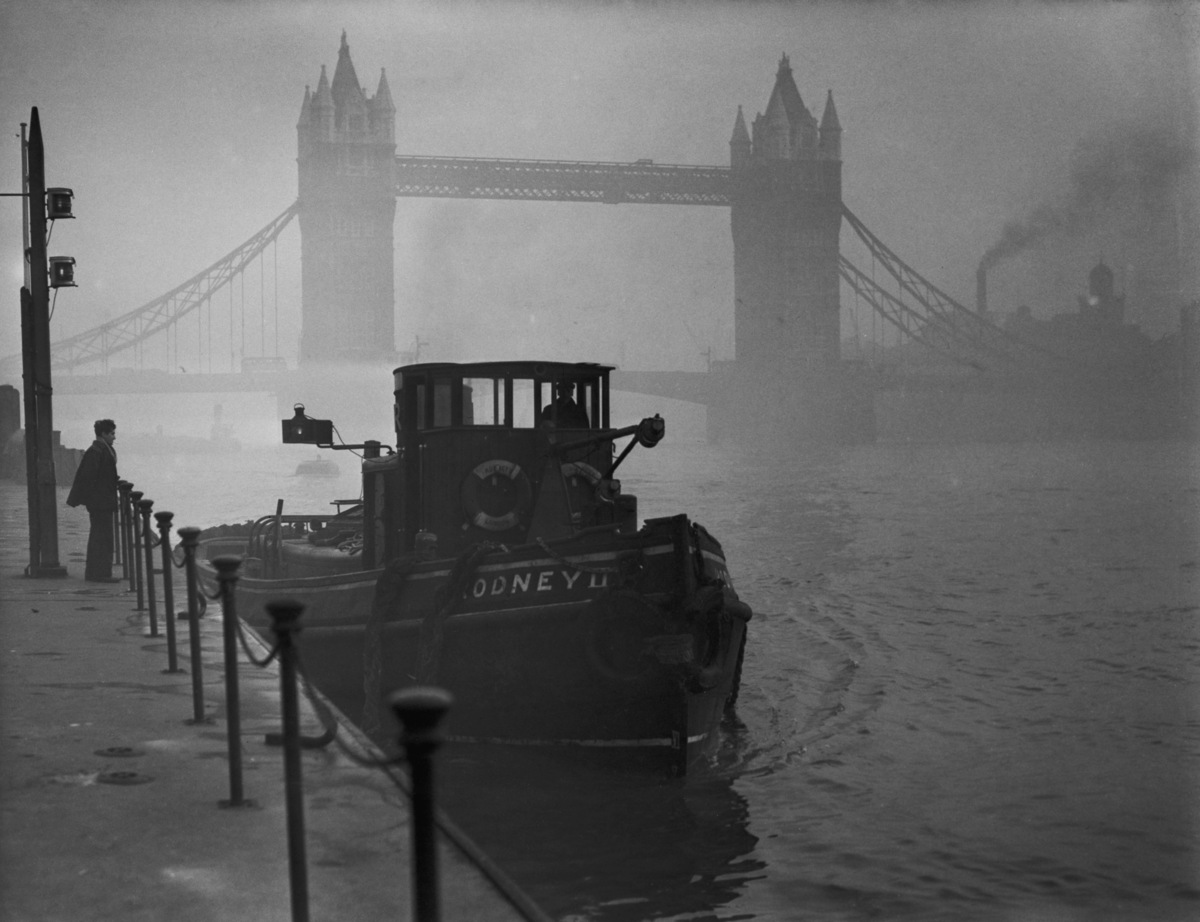
\includegraphics[scale=.8]{images/great_smog.jpg}
  \caption[Great smog of 1952]{Great smog of 1952 \cite{ElliotWagland2013}}
  \label{fig:interaction_design}
\end{figure}

One historic event which caused huge consequences is known as the great smog of 1952. Thousands of people died in Greater London due to exposure over several days to a highly contaminated atmosphere, and many others became ill or experienced retarded symptoms \cite{Bell2008}. The fog originated from coal burning, vehicle exhaust and other atmospheric factors. Although many human activities introducing pollution have changed since then, it became evident the immediate and retarded health impact of pollution. 

Pollution particles can be categorised into gaseous pollutants, persistent organic pollutants, heavy metals and particulate matter. They vary in their chemical composition, emission sources and impact on health. 

Gaseous pollutants are sulphur dioxide (\SOTWO), nitrogen oxides (\NOX), carbon monoxide (CO), ozone (\OTHREE) and volatile organic compounds (VOCs). The principal source of gaseous pollutants is combustion of fossil fuels and diesel emission from vehicles. Nitrogen oxides (\NOX) is a general term that includes nitric oxide (NO) and nitrogen oxide \NOTWO. Gaseous pollutants can affect our health by inflaming the airways and lungs, and in the long term, affect the function of the lungs \cite{AirQualityExpertGroup2004} \cite{WHO2003}.

Particulate matter (PM) is a mixture of solid and liquid particles (such as sulphate, nitrates, ammonia, sodium chloride, black carbon, mineral dust and water). PM are categorised according to their diameter size measured in microns (\SI{}{\micro\metre}, one millionth of a metre). Particles smaller than 10 microns (\PMTEN) are known as coarse particles, smaller particles with a size of up to 2.5 and 1 microns (\PMTWO and \PMONE) are known as fine and ultra-fine particles respectively. They are differentiated in sizes because it dictates their aerodynamic properties, that is, how they are transported into the air, as well as how far they can get into the respiratory system. According to the World Health Organization, PM is the most harmful pollutant because it can pass through the nose and throat and enter the lungs, there is also evidence that it is associated with risk of cardiovascular disease \cite{Polichetti2009}. 

Air quality is also affected by pollution mixture in further complex chemical structures and by temperature and humidity conditions. \NOTWO, PM and O\textsubscript{3}  pollutants get transformed by atmospheric processes making it hard to evaluate their individual impact. As an example, ground level ozone is produced when sunlight interacts with \NOTWO and volatile organic compounds. Furthermore, \NOTWO and other nitrogen oxides also contribute to PM generation, making \NOX a particularly concerning pollutant.

\subsection{Air quality data dissemination}
Openly published air quality data aimed to have informed and aware citizens that could take part into more sustainable and environmental choices. \quotes{Yet, what was lacking (and it still is), is a model for effective communicating of environmental information to the public} \cite{Thinh2007}. Terms like assessment, limit values, target values and concentration, among others, are commonly used by air quality data publishers to describe the current or forecasted quality status; however, there is not general agreement on how air quality information should be disseminated to the general public in a way it is understood immediately and intuitively. 

In general it is complex to categorise and establish measures for the different components of air pollution due their heterogeneous nature and the chemical reactions that occur between them. Measurement methods and units vary from institution to institution and regulation standards can be specific for each country, which may give rise to ambiguity. Furthermore, much of the available data is represented in a tabular format, including various information for individual pollutants, as exemplified in table \ref{tab:pollution_tabular_data}. This table was extracted from the  Department for Environment Food and Rural Affairs (DEFRA) website \cite{DepartmentforEnvironmenta}, and shows measures related to the air quality from a sensing station located in Deaconess Garden in the south of Edinburgh. At first sight it table arises some questions for the novice on air-quality trying to crack the data. Firstly, the pollution codes such as PM2.5, PM10, NO2, NOX as NO2 and their subtle differences should be understood. Secondly, some measurement units are tagged with the monitoring method used to extract the information, like the TEOM FDMS \footnote{Which indicates that the sensing methods were Tapered Element Oscillating Microbalance and Filter Dynamics Measurement System \cite{Quality2005}} tag. And lastly, it is hard to know which measurements are of more interest given a person's particular circumstances. As stated by Brimblecombe and Schuepbach \cite{P.Brimblecombe2008}, \quotes{many people complain that the information is unintelligible, while some have even seen it as an attempt of government to blind the public with science}.  It is clearly difficult to understand the meaning of the terms and values that are used to represent air quality data to the general public. 

\begin{table}[ht]
\centering
\begin{adjustbox}{width=1.2\textwidth,center=\textwidth}
\begin{tabular}{rlrrrrrrr}
  \hline
 Pollutant & Date & Time & Measurement & Unit & Period & Comment  \\ \hline
    Ozone (O3) & 20/07/2016 & 07:00 & 63.06412 & µg/m3 & Hourly & - \\
    Nitric oxide (NO) & 20/07/2016 & 07:00 & 2.61933 & µg/m3 & Hourly & - \\
    Nitrogen dioxide (NO2) & 20/07/2016 & 07:00 & 27.34875 & µg/m3 & Hourly & - \\
    Nitrogen oxides as nitrogen dioxide (NOXasNO2) & 20/07/2016 & 07:00 & 31.36500 & µg/m3 & Hourly & - \\
	Sulphur dioxide (SO2) & 20/07/2016 & 07:00 & 14.63495 & µg/m3 & Hourly & - \\
	Carbon monoxide (CO) & 20/07/2016 & 07:00 & 0.081494 & mg/m3 & Hourly & - \\
	PM10 particulate matter (Hourly measured) (PM10) & 18/07/2016 & 15:00 & 10.900 & µg/m3 (TEOM FDMS) & Hourly & - No current data. \\
	Non-volatile PM10 (Hourly measured) (Non-volatile PM10) & 19/07/2016 & 07:00 & 26.700 & µg/m3 (TEOM FDMS) & Hourly & - No current data. \\
	Volatile PM10 (Hourly measured) (Volatile PM10) & 19/07/2016 & 07:00 & 5.500 & µg/m3 (TEOM FDMS) & Hourly & - No current data. \\
	PM2.5 particulate matter (Hourly measured) (PM2.5) & 18/07/2016 & 15:00 & 4.300 & µg/m3 (TEOM FDMS) & Hourly & - No current data. \\
	Non-volatile PM2.5 (Hourly measured) (Non-volatile PM2.5) & 19/07/2016 & 07:00 & 16.300 & µg/m3 (TEOM FDMS) & Hourly & - No current data. \\
	Volatile PM2.5 (Hourly measured) (Volatile PM2.5) & 19/07/2016 & 07:00 & 5.000 & µg/m3 (TEOM FDMS) & Hourly & - No current data. \\
	Modelled Wind Direction (Dir) & 19/07/2016 & 24:00 & 50.6 & \degree & Hourly & - No current data. \\
	Modelled Wind Speed (Speed) & 19/07/2016 & 24:00 & 6.2 & m/s & Hourly & - No current data. \\
	Modelled Temperature (Temp) & 19/07/2016 & 24:00 & 14.6 & °C & Hourly & - No current data. \\
	PM10 Ambient Temperature (AT10) & 19/07/2016 & 07:00 & 19.4 & °C & Hourly & - No current data. \\
	PM10 Ambient pressure measured (AP10) & 19/07/2016 & 07:00 & 989.0 & mb & Hourly & - No current data. \\
	PM2.5 Ambient Temperature (AT25 ) & 19/07/2016 & 07:00 & 17.5 & °C & Hourly & - No current data. \\
	PM2.5 Ambient Preasure (AP25) & 19/07/2016 & 07:00 & 988.0 & mb & Hourly & - No current data. \\
   \hline
\end{tabular}
\end{adjustbox}
\caption{Air quality tabular data representation. \cite{DepartmentforEnvironment}}
\label{tab:pollution_tabular_data}
\end{table} 

\subsection{The COMEAP air quality index and health advice}
In order to understand the correlation between air quality data and its effects on human health, the Committee on the Medical Effects of Air Pollutants (COMEAP) developed the air quality index based on health evidence. It is used to communicate real-time air quality levels and their short-term health effects for five selected harmful pollutants: particulate matter (\PMTEN and \PMTWO), ozone (\OTHREE), sulphur dioxide (\SOTWO), and nitrogen dioxide (\NOTWO) as shown in Figure \ref{fig:air_quality_index}. The index employs a colour scale and a number index to inform about how high are the concentrations of each specific pollutant. Four bands are employed: Low, Moderate, High and Very High. 

\begin{figure}[H]
\begin{adjustbox}{width=1\textwidth,center=\textwidth}
  \centering
  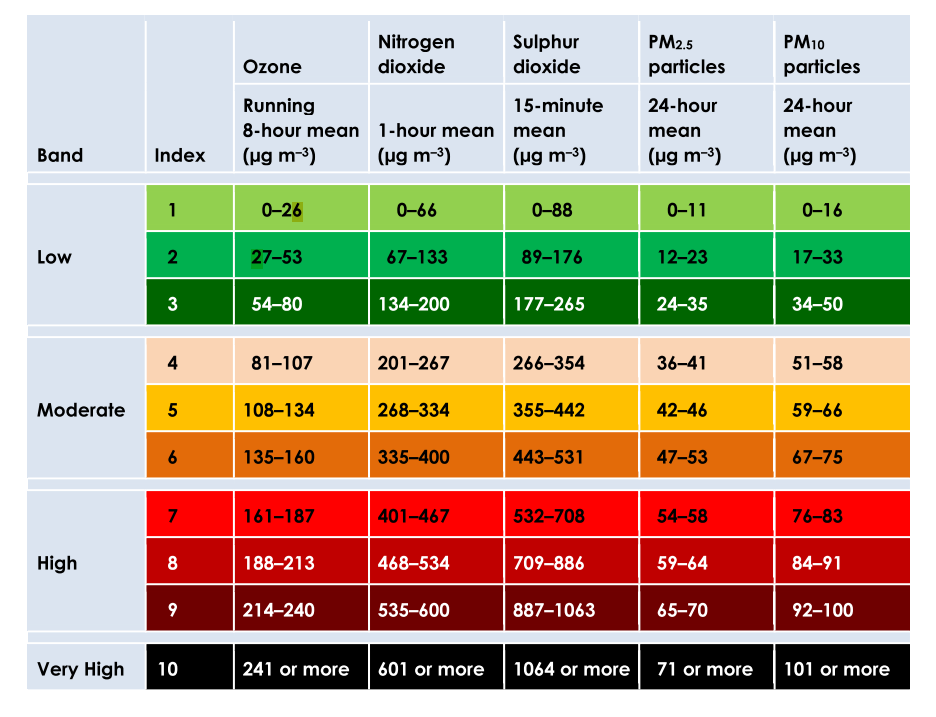
\includegraphics[scale=.8]{images/air_quality_index.png}
\end{adjustbox}
  \caption[The COMEAP air quality index]{The COMEAP air quality index \cite{HealthProtectionAgencyfortheCommitteeontheMedicalEffectsofAirPollutants2011}}
  \label{fig:air_quality_index}
\end{figure}

There is substantial evidence that the elderly, children, and persons that suffer from chronic diseases such as asthma are in greater danger of suffering symptoms and health consequences from lower pollution concentrations than the general public \cite{Koenig1999} \cite{Kampa2008} \cite{Zones2010} . The COMEAP includes such population in their Air Quality Index to give them the opportunity to modify their behaviour and reduce the severity of their symptoms. Furthermore, the air quality index is accompanied by a health advice (Figure \ref{fig:air_quality_health_advice}) which provides specific health messages targeting both population groups, sensitive and non-sensitive providing information about the actions that should be taken to avoid symptoms and health effects.

\begin{figure}[H]
\begin{adjustbox}{width=1\textwidth,center=\textwidth}
  \centering
  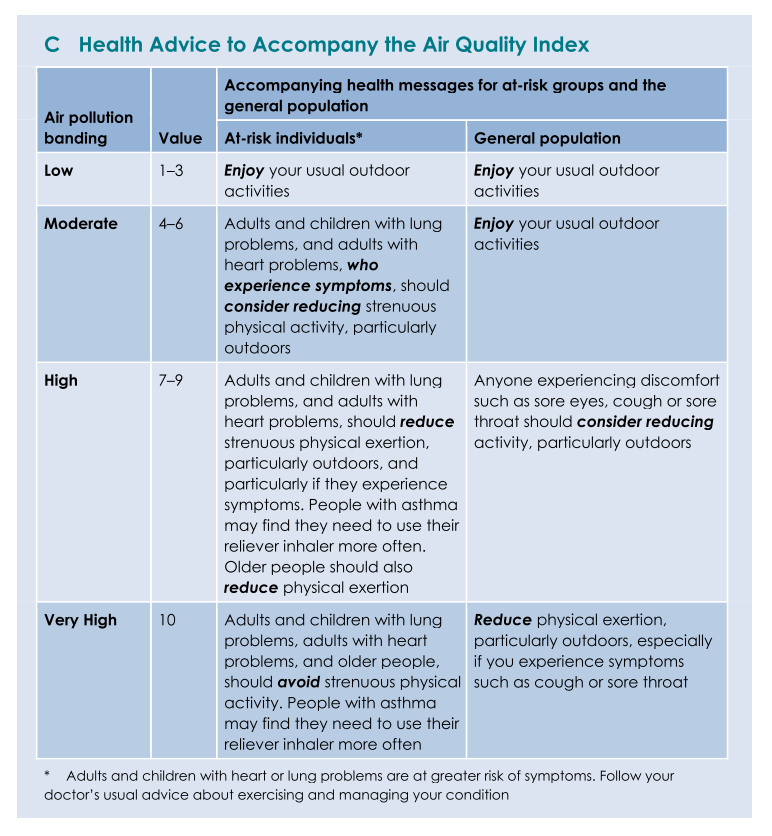
\includegraphics[scale=.8]{images/air_quality_health_advice.png}
\end{adjustbox}
  \caption[Air quality health advice]{Air quality health advice \cite{HealthProtectionAgencyfortheCommitteeontheMedicalEffectsofAirPollutants2011}}
  \label{fig:air_quality_health_advice}
\end{figure}


\subsection{Air quality sensors}

\begin{itemize}

\item Fixed sensors: 

Fixed sensors are installed and maintained by the UK government and local authorities in Scotland. There are of two kinds, automatic sensors from the Automatic Urban and Rural Network (AURN)\footnote{\url{https://uk-air.defra.gov.uk/networks/network-info?view=aurn}}, and non automatic sensors maintained by local Scottish councils. 

	\begin{itemize}
    
    \item Automatic sensors: They produce hourly concentrations and data is sent automatically over the network. They purpose is to check that EU and other regulatory standards are being met as well as informing the public about air quality. These sensors monitor a wide range of pollutants (\NOX, \SOTWO, CO\textsubscript{2}, O\textsubscript{3}, \PMTWO and \PMTEN) which are later collected and processed by Ricardo Energy and Environment \footnote{\url{http://ee.ricardo.com}} and exposed through HTML webpages at the Scottish Air Quality website\footnote{\url{http://www.scottishairquality.co.uk/}} or CSV files provided on demand. 
	\item Non automatic sensors: 
    
    \end{itemize}

\item Portable sensors:

\item Participatory sensors:

Some projects such as CitiSense \cite{Nikzad2012} include users as 'human sensors' by reading their perceptions towards air quality in certain locations. This method aims to get more fine-grained information about air quality and engage the citizens in the pollution problem and its solution. 

\end{itemize}




\section{Data visualisation}

\subsection{Definition}
A number of definitions have been proposed to explain what data visualisation means. According to Friendly \cite{Friendly2009} the term came together with the birth of statistical thinking as a way to illustrate mathematical language, their trends, tendencies and distributions through the use of diagrams and graphics. Few \cite{StephenFew2013} describes it as a graphical display of abstract information for the purpose of sense-making and communication. 
However, this definition does not exclude representations that are not algorithmically drawn. The definition offered by Iliinsky and Steele \cite{Iliinsky2011} is more specific: 
\begin{displayquote}
Any visual representation of data that is:
	\begin{itemize}
	\item algorithmically drawn (may have custom touches but is largely rendered with the help of computerized methods);
	\item easy to regenerate with different data (the same form may be repurposed to represent different datasets with similar dimensions or characteristics);
	\item often aesthetically barren (data is not decorated); and
	\item relatively data-rich (large volumes of data are welcome and viable, in contrast to infographics).
    \end{itemize}
\end{displayquote}
\iffalse
\begin{figure}[h]
  \centering
  \begin{adjustbox}{width=.8\textwidth,center=\textwidth}
  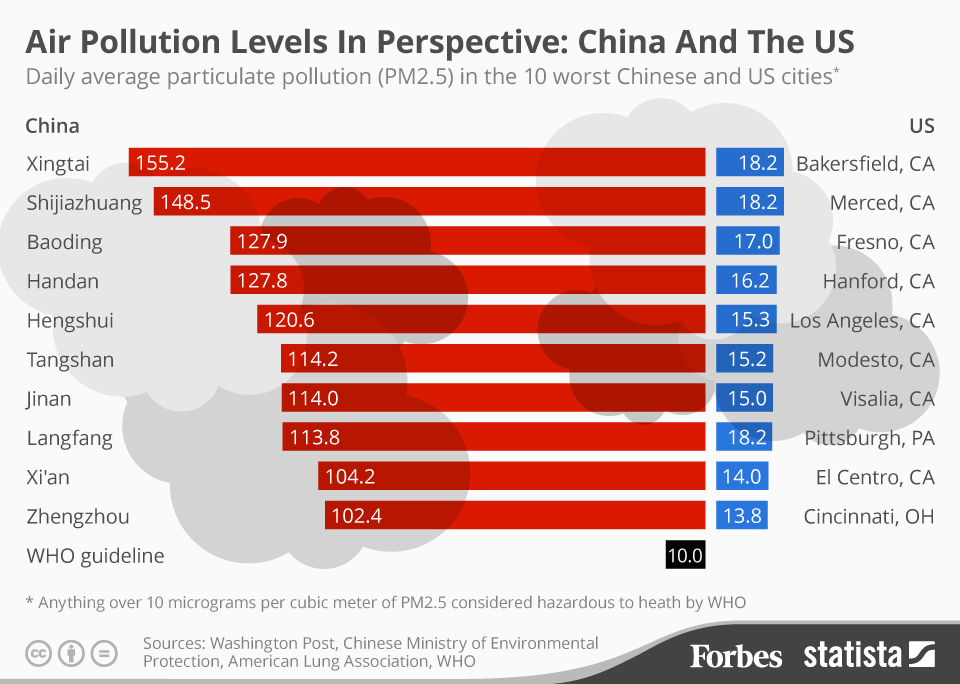
\includegraphics[scale=1]{images/air_pollution_infographic.jpg}
  \end{adjustbox}
  \caption[Air pollution infographic]{Air pollution infographic \cite{NiallMcCarthy}}
  \label{fig:air_pollution_infographic}
\end{figure}
\fi
A visualisation helps in the understanding of data  by taking advantage of the human visual system to process a large amount of information quickly, thus allowing the human brain to identify patterns, links and relationships between the represented objects. Daniel et al. \cite{KeimDaniel2010}, also states that visualising enables people to: 
\begin{displayquote}
	\begin{itemize}
\item  Synthesise information and derive insight from massive, dynamic, ambiguous, and often conflicting data.
\item Detect the expected and discover the unexpected.
\item Provide timely, defensible, and understandable assessments.
\item Communicate these assessment effectively for action.
	\end{itemize}
\end{displayquote}

Data visualisation is essential when the available data is vast and dynamic, and when raw data does not make sense on its own. Therefore, data must be encoded using technological and design elements;  potentially making use of disciplines such as statics, data mining, human computer interaction and graphic design. 

\subsection{Designing data visualisations}
Figure \ref{fig:data_visualization_process} depicts the visual analysis process according to Daniel et al. \cite{KeimDaniel2010}. In the first stage,  data should be collected, usually from many distinct data sources and standardised into one common format. This later enables to choose between the creation of models, or visualisations. Models are an automated representation that requires data mining techniques whereas visualisations are manual representations that can be created through simple mapping from data to the visual context. Both representations are linked together to enable validation and refinement through iteration. The final stage is arguably the most important as it is concerned with the knowledge gained from the representation and aims to respond the questions posed from the study in the first place.
\begin{figure}[!htb]
\begin{adjustbox}{width=1\textwidth,center=\textwidth}
  \centering

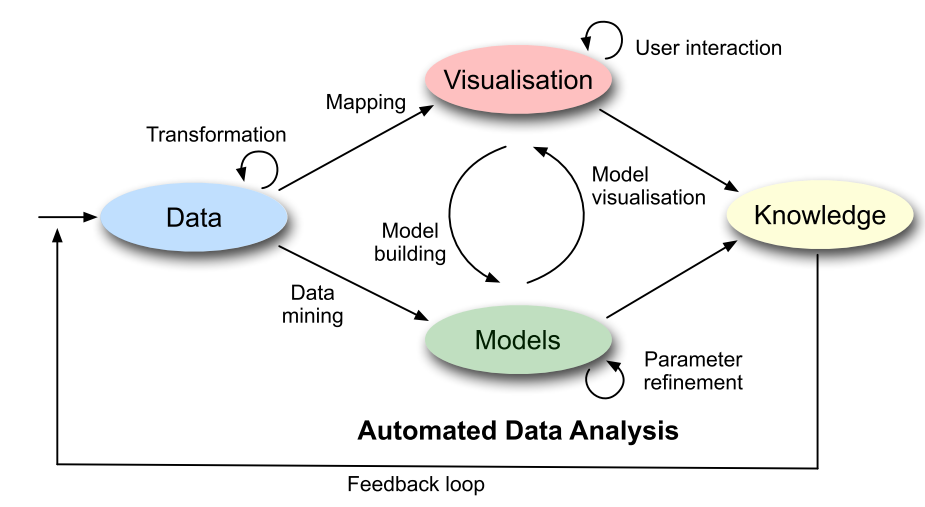
\includegraphics[scale=1]{images/data_visualization_process.png}
\end{adjustbox}
  \caption[The data visualisation process]{The data visualisation process \cite{KeimDaniel2010} }
  \label{fig:data_visualization_process}
\end{figure}

According to Ben Fry \cite{Cleveland1993}, one specific approach for data visualisations is illustrated in Figure \ref{fig:data_visualization_stages}, which establishes a common series of steps that can be followed for this purpose:

\begin{displayquote}
	\begin{itemize}
\item Acquire: Obtain the data, whether from a file on a disk or a source over a network. 
\item Parse: Provide some structure for the data’s meaning, and order it into categories. 
\item Filter: Remove all but the data of interest. 
\item Mine: Apply methods from statistics or data mining as a way to discern patterns or place the data in mathematical context.
\item Represent: Choose a basic visual model, such as a bar graph, list, or tree. 
\item Refine: Improve the basic representation to make it clearer and more visually engaging. 
\item Interact: Add methods for manipulating the data or controlling what features are visible.
\end{itemize}
\end{displayquote}

\begin{figure}[!htb]
\begin{adjustbox}{width=1\textwidth,center=\textwidth}
  \centering
  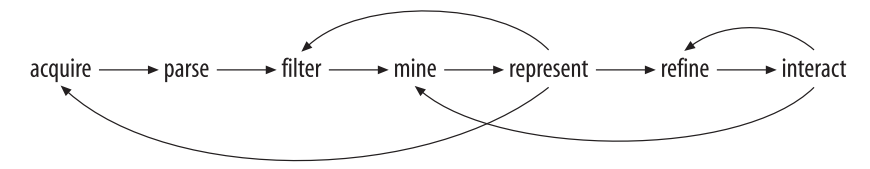
\includegraphics[scale=1]{images/visualization_stages.png}
\end{adjustbox}
  \caption[Visualisation stages]{Visualisation stages  \cite{Cleveland1993} }
  \label{fig:data_visualization_stages}
\end{figure}
From this perspective, it is possible to establish that all visualisations require an elemental process guided by the designer to enable the recognition of patterns within the data. Also that the design process is an iterative task where the designer may go back to redefine any stage of the process until the desired result is achieved. 

\subsection{Data visualisations for decision support}
Caroll, Anderson, Olson et al established in their analysis of human-computer interaction that
\quotes{a decision-making process usually includes the acquisition of related information, the construction of a mental representation of the problem and solutions, and the identification of an optimal solution} \cite{carroll1987mental} as cited in \cite{Zhu2008}, decision making involves acquiring domain-specific information about a particular question which is the intended output of a data visualisation. Therefore, it is important to understand the effects of data visualisations in decision support.

The decision-making process takes into account the decision maker's skill, the task of making a decision and the problem space. In our specific context, the decision maker should be able to understand the data in its represented space (visualisation), evaluate the problem (avoid air pollution) and execute a decision task (leave the polluted space). \quotes{A well-designed visualisation takes features of the decision task and the characteristics of the decision makers into consideration} \cite{Zhu2008}. Thus, visualisations should be created in the specific context of the decision makers; discovering beforehand the knowledge they should have; the problems they are likely to face; and the potential decisions they should be able to make. 

\section{Air quality visualizations}
The problem of making the air quality problem visible to the general population has been addressed before, from map based representations, to wearable devices and in-city displays. These approaches contemplate new or known was to tackle the problem of air quality, and therefore; making the invisible visible.

\subsection{Table based}
The most basic representation of air quality data is as tabular data, generally including some colors to indicate the quality level of the measurement as shown in figure \ref{fig:table_based_visualization}. From these kind of representations is easy to read information from multiple places when the user is familiar to the values. But, as stated before, this representations have many drawbacks. 

\begin{figure}[H]
\begin{adjustbox}{width=1\textwidth,center=\textwidth}
  \centering
  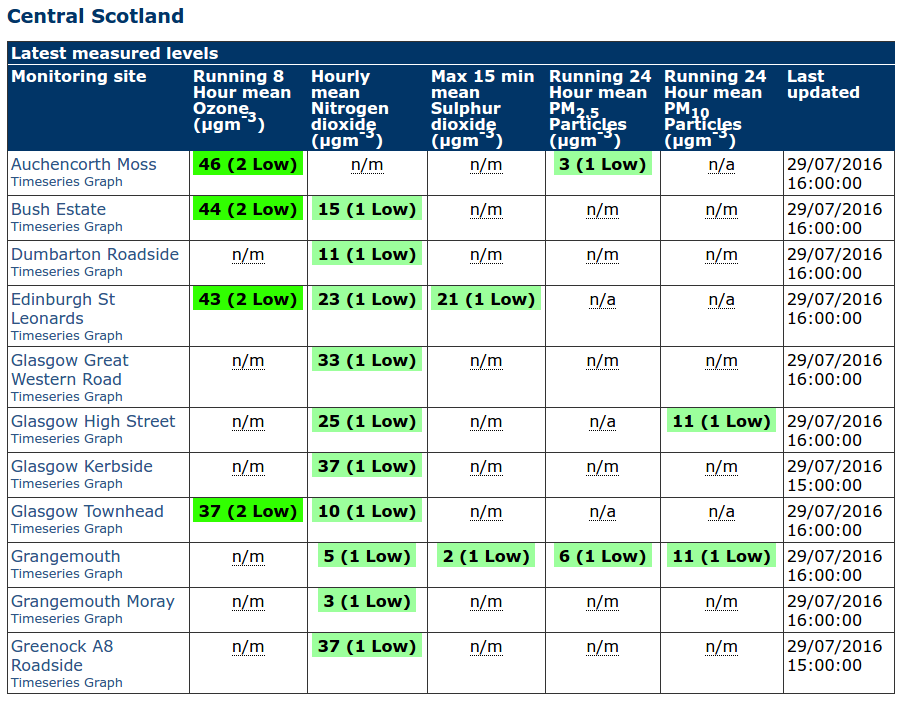
\includegraphics[scale=1]{images/tabular_data.png}
\end{adjustbox}
  \caption[Tabular visualization]{Tabular visualization \cite{DepartmentforEnvironment}}
  \label{fig:table_based_visualization}
\end{figure}

\subsection{Map based}
Through maps; people is able to understand where the measurements are coming from. Some representations include color indicators to show how good or bad the measurements are. However; it is unlikely that one is interested in the measurements for all Scotland's regions, it is time consuming to browse manually to the desired zone to explore the current values and it is hard to correctly visualize overlaid numeric data on small screens.

\begin{figure}[H]
\begin{adjustbox}{width=1\textwidth,center=\textwidth}
  \centering
  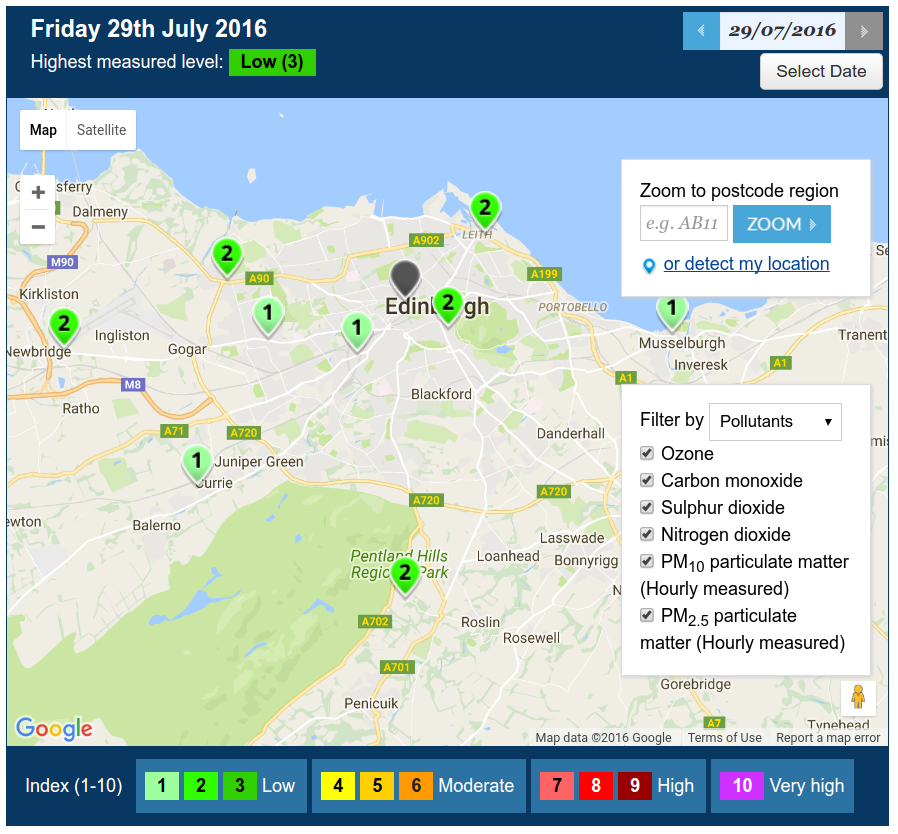
\includegraphics[scale=.30]{images/map_visualization.png}
\end{adjustbox}
  \caption[Map-based visualization]{Map-based visualization \cite{Scottishairquality.co.uk2016}}
  \label{fig:web_based_desktop_visualization}
\end{figure}


\subsection{Line based}
The inAir project \cite{Kim2013} utilizes a line graph to represent indoor particle matter count over a defined period of time. Their findings suggested that this approach enables users to reflect on their behaviors and air quality status, persuading them to modify their practices to decrease their exposure to air pollution.

\begin{figure}[H]
\begin{adjustbox}{width=1\textwidth,center=\textwidth}
  \centering
  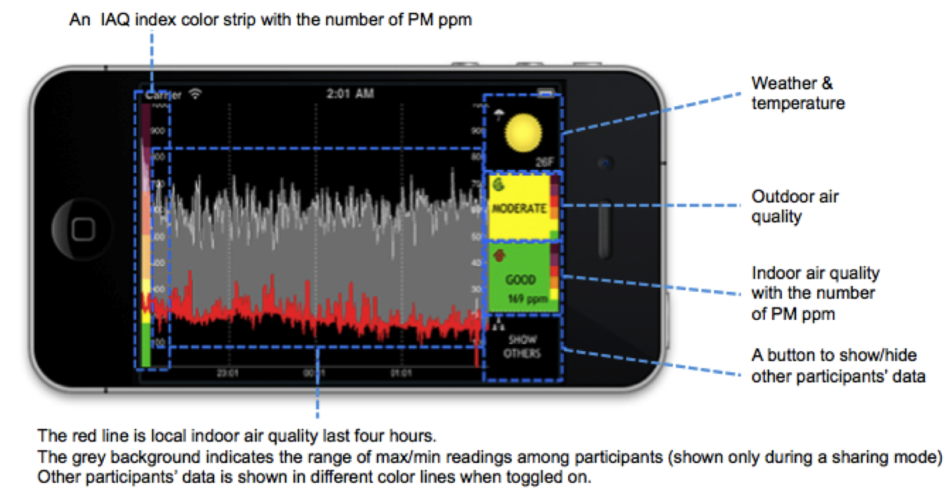
\includegraphics[scale=1]{images/InAir.png}
\end{adjustbox}
  \caption[inAir project: line-based visualizations]{inAir: line-based visualization\cite{Kim2013}.}
  \label{fig:line_based_inAir}
\end{figure}


\subsection{Photo based}
Photo-based representations as proposed by Lin \cite{Lin2014}, allow people to understand levels of pollution by taking pictures of the current environment. The pictures are later adjusted using a filter that represents the air quality status (NO2) at that location. This serves as a playful and habitual way to visualize air quality. On the other hand, this project only aggregates nitrogen dioxide readings, excluding other pollutants that may be pertinent, as well as not going further to indicate what should a person do given the pollution levels.

\begin{figure}[H]
\begin{adjustbox}{width=.8\textwidth,center=\textwidth}
  \centering
  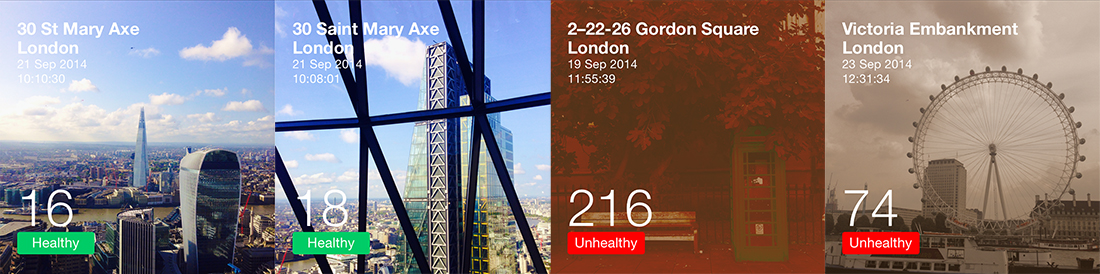
\includegraphics[scale=.4]{images/instaNO2.jpg}
\end{adjustbox}
  \caption[InstaNO2 project: photo-based visualizations]{InstaNO2: photo-based visualizations \cite{Lin2014}.}
  \label{fig:photo_based_instaNO2}
\end{figure}

\subsection{Tangible approaches}
Other approaches have made use of tangible objects to visualize air pollution in a more engaging way. The Human sensor project \cite{InvisibleDust2016} employs wearable art and in-city performances to reveal changes in pollution. Similarly, WearAir \cite{Kim2010}, is an expressive T-shirt that senses VOCs and expresses the readings making use of embedded lights. Kuznetsov et al. \cite{Kuznetsov2011} developed glowing balloons with air quality sensors for users to explore urban air quality. The IBM think exhibit \cite{IBM2012} is a 123-foot long digital wall display located in New York city which renders art patterns and real time streaming visualizations showing air quality data as well as traffic flow, energy, and water usage. This is intended to be an immersive in-city experience for users to explore and understand the role of data in the world. Tangible approaches are useful because the evoke curiosity and surprise while gaining an insight of what is happening. In contrast, they are not intended for personal day to day usage but as a way of expression and art. 

\begin{figure}[H]
\begin{adjustbox}{width=.8\textwidth,center=\textwidth}
  \centering
  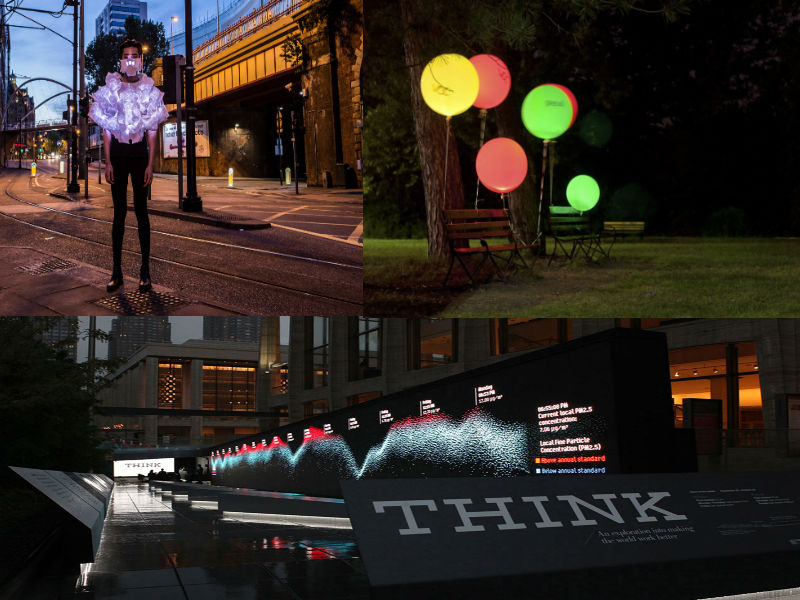
\includegraphics[scale=.4]{images/think_human_sensor_balloons.jpg}
\end{adjustbox}
  \caption[Tangible visualizations]{The human-sensor on the top-left \cite{InvisibleDust2016}, glowing balloons on the top-right \cite{Kuznetsov2011}, and IBM think on the bottom \cite{IBM2012}.}
  \label{fig:photo_based_instaNO2}
\end{figure}


\section{Mobile applications}
In recent years mobile applications are becoming increasingly popular in many domains, such as business, health and entertainment. According to the 2015 mobile app report \cite{ComScore}, the time spent on mobile devices grew up from 51 percent in share spent time to a 62 percent, leaving the share spent time of desktop on a 38 percent and becoming the number one of digital media consumption in 2015. Also, the usage of apps which include health or tracking functions was unknown until 2014, when several apps experienced a huge grow of up to 922 percent each year. 

\subsection{Personal applications and new hardware capabilities}

Mobile devices have reached a point where their hardware capabilities are comparable to a desktop computer capabilities regarding their processing power and available RAM; furthermore, they provide added functions that are unimaginable for a desktop computer, such as GPS, accelerometer; and the ability to be carried throughout the day. This enables new ways of living and interacting with technology as well as bringing closer the idea of ubiquitous computing, "perhaps ubiquitous computing is already here, but took a form other than that which had been envisioned." \cite{Bell2007}. 

\begin{figure}[h]
\begin{adjustbox}{width=.4\textwidth,center=\textwidth}
  \centering
  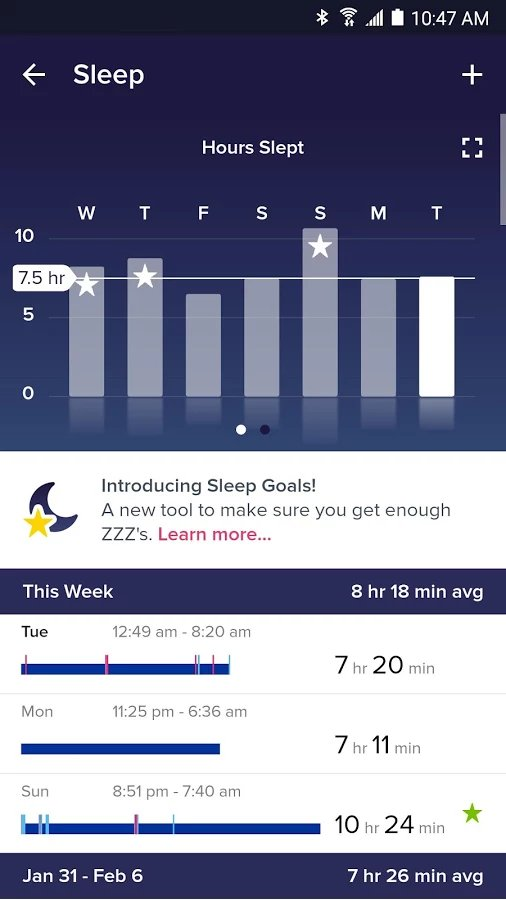
\includegraphics[scale=.5]{images/sleep_tracking.jpg}
\end{adjustbox}
  \caption[Fitbit application sleep tracking]{Fitbit application sleep tracking \footnote{\url{https://www.google.com/fit/}}}
  \label{fig:google_fit}
\end{figure}

Example of emerging applications that heavily rely on new devices hardware's capabilities, are Google Fit \footnote{\url{https://www.google.com/fit/}}, Nike + \footnote{\url{http://www.nike.com/us/en_us/c/nike-plus/running-app-gps}}, Fitbit \footnote{\url{https://www.fitbit.com/uk}} Jawbone Up \footnote{\url{https://jawbone.com/up}} and Garmin Connect \footnote{\url{https://connect.garmin.com/en-US/}}. These apps make use of sensors that although simple and cheap; are able to measure a range of activities carried out by a person. Such activities go from time and quality of sleep, calories ingested during the day, average heart rate of a run or steps taken during a city walk that according Morrison et al. \cite{Rooksby2014},  allows to count and measure areas of a person's life to optimize behavior as desired.

Recent research \cite{Barkhuus2011} suggests that people uses mobile applications in personalized or individual manners, adapting functions to meet their priorities; adding  new functions to create their own unique experiences based on their everyday lives. There is an enormous opportunity for crafting new applications that not only can give unique and valuable experiences; but influence the way people do things in the real world. 

\subsection{Challenges and usability considerations}

Core differences between desktop and mobile applications make mobile development more challenging than desktop development \cite{Chittaro2006}. Important examples of this that should be accounted when designing visualizations for mobile devices are, among others; limited processing power, smaller screen, multiple types of screens and slower connectivity. This issues become evident when trying to translate a visualization such as the shown in 
\iffalse
\ref{fig:web_based_desktop_visualization}, 
\begin{figure}[h]
\begin{adjustbox}{width=1.2\textwidth,center=\textwidth}
  \centering
  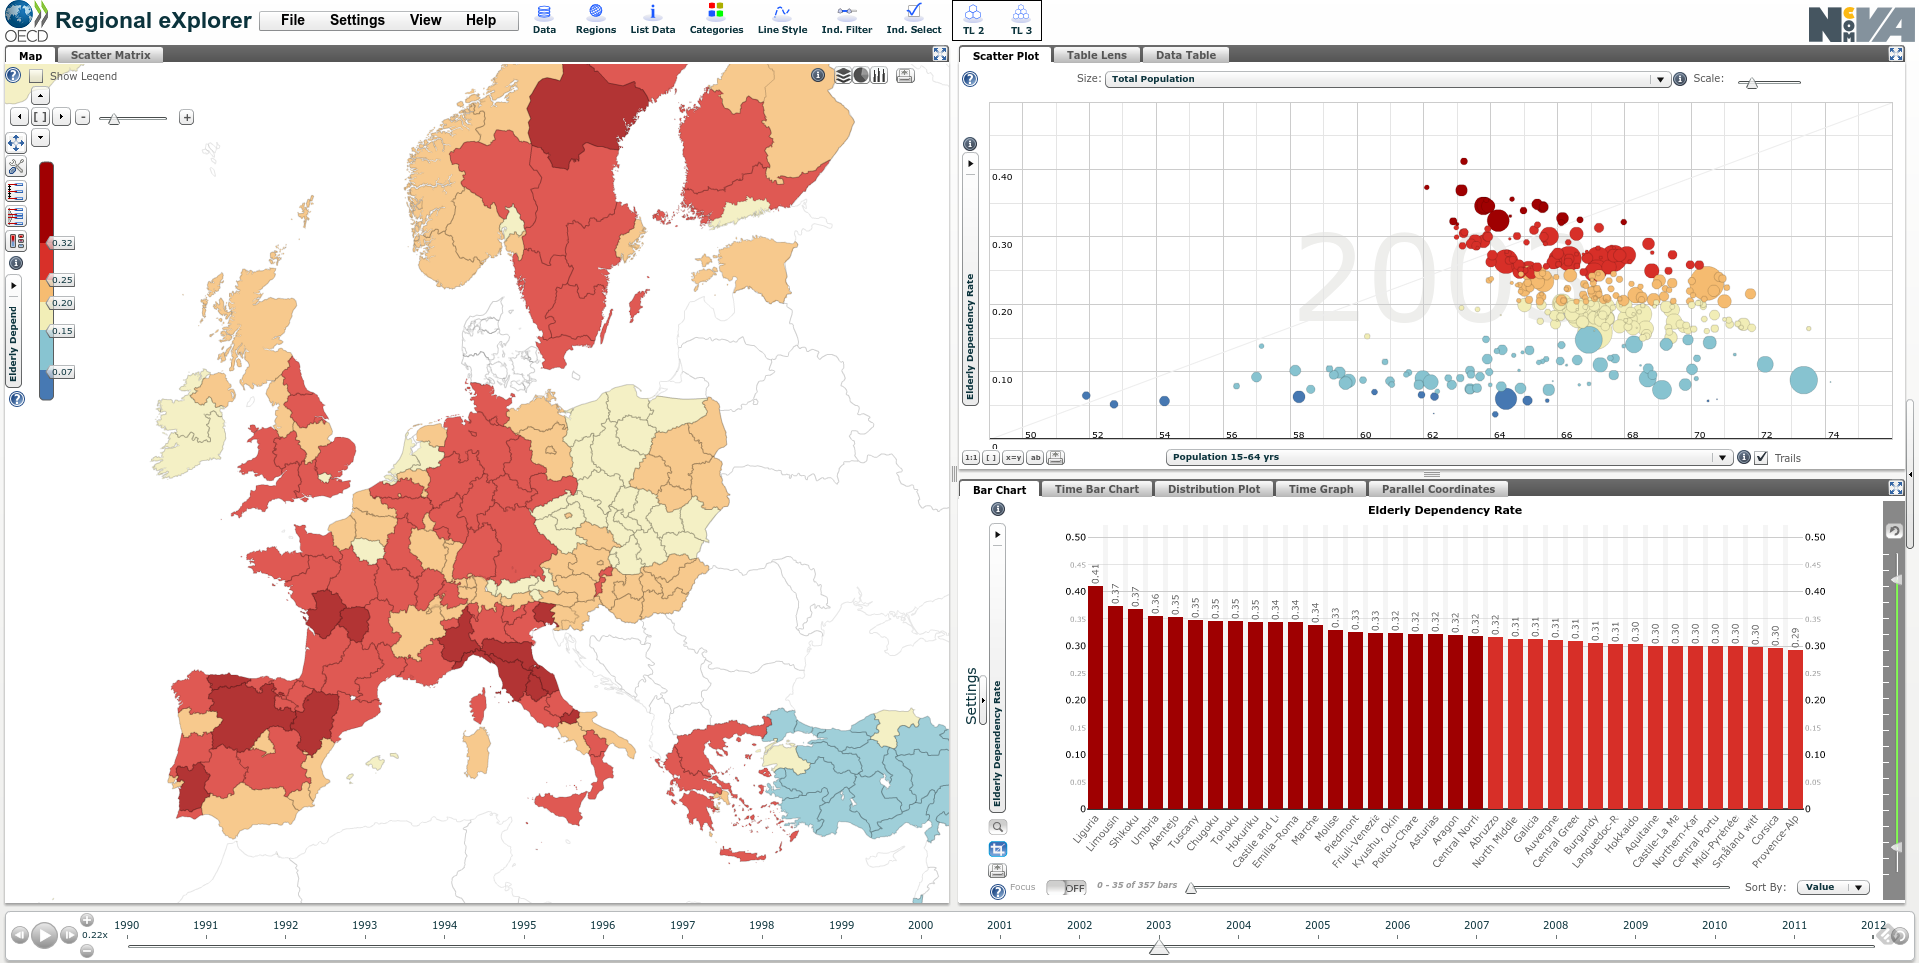
\includegraphics[scale=.5]{images/visualization_desktop_example.png}
\end{adjustbox}
  \caption[Line-based visualization]{Line-based visualization}
  \label{fig:web_based_desktop_visualization}
\end{figure}
\fi
It is particularly challenging to design mobile applications in contrast to desktop applications because 

(PEND)





\iffalse
\section{Air quality sites and applications}
Currently there are several air-quality related web or mobile applications. In order to understand how to create a new application
with added value and functionalities, a review on existing applications or was carried out. Due to limited time, this search was restricted to software working in Scotland on Android devices or web browsers. More specifically, the more popular websites and android applications in the market and in search engines were analyzed.
The following table illustrates the functions that are currently offered by this applications or websites. 

\begin{itemize}
	\item F1 (Air quality info in general)
	\item F2 (Air quality in many locations)
    \item F3 (Air quality in current location)
    \item F4 (Air quality in form of a map)
    \item F5 (Pollution indicators)
	\item F6 (Notifications)
    \item F7 (Changes over time)
	\item F8 (Forecast)
    \item F9 (Personal sensor)
\end{itemize}

\begin{table}[ht]
\centering
\begin{adjustbox}{width=1.2\textwidth,center=\textwidth}
\begin{tabular}{rlrrrrrrrrrr}
  \hline
 Name & Type & Description & F1 & F2 & F3 & F4 & F5 & F6 & F7 & F8 & F9 \\ \hline
    \url{http://www.scottishairquality.co.uk/} & Website & Air quality status and forecasts offered by the Scottish Government & - & X & X & X & X & X & X \\
    \url{http://www.environment.scotland.gov.uk/} & Website & Air quality status and forecasts offered by the Scottish Government & - & X & X & X & X & X & X \\
    \url{http://www.environment.scotland.gov.uk/} & Website & Air quality status and forecasts offered by the Scottish Government & - & X & X & X & X & X & X \\
    \url{http://www.environment.scotland.gov.uk/} & Website & Air quality status and forecasts offered by the Scottish Government & - & X & X & X & X & X & X \\    

   \hline
\end{tabular}
\end{adjustbox}
\caption{Air quality tabular data representation. \cite{DepartmentforEnvironment}}
\label{tab:pollution_tabular_data}
\end{table} 
\fi



\section{Issues and current needs}
From outlining why pollution matters, its relevance to different population groups and the use of visualization to convey relevant data, the limitations of current approaches as a means of communication become apparent. Current approaches fail to take into account the general population and sensitive pollution users according to the COMEAP. There is the need for a tool that includes both user groups and their personal circumstances in order to provide more accurate information for the purpose of decision making. It was also outlined how apps are enabled to create new enhanced personal experiences being an appropriate vehicle to achieve such need.
